\documentclass[portrait,a0]{a0poster}

\RequirePackage[utf8]{inputenc}  
%\usepackage[utf8]{inputenc}  
%\usepackage[francais]{babel} 
\usepackage[pdftex]{color,graphicx}   % paquetage graphique : pdftex
\DeclareGraphicsExtensions{.jpg,.pdf,.mps,.png} % type de fichiers graphiques supportes par graphicx
\usepackage[pdftex,bookmarks=true,colorlinks=true]{hyperref} % liens hypertext
%\usepackage[latin1]{inputenc}
\usepackage{amsfonts}
\usepackage{amsmath}
\usepackage{amssymb}
\usepackage{paralist}
\usepackage{balance}
% couleur des liens
%\hypersetup{colorlinks, citecolor=black, filecolor=black, linkcolor=black, urlcolor=black}
\hypersetup{colorlinks, citecolor=black}

\usepackage{multicol}
\usepackage{paralist}
\usepackage{pgf}
\usepackage{pgfcore}
\usepackage{pgfbaseimage}
\usepackage{pgfbaselayers}
\usepackage{pgfbasepatterns}
\usepackage{pgfbaseplot}
\usepackage{pgfbaseshapes}
\usepackage{pgfbasesnakes}
\usepackage{tikz}
\usetikzlibrary{shapes,arrows}
\usepackage{amssymb}
\usetikzlibrary{backgrounds} % a partir de la version 1.18 de PGF
\usepackage{everyshi,eso-pic,calc,ifthen,wallpaper} %%  this is for using an image as background . . .
\usepackage{url}
\usepackage{fancybox}
\usepackage{sectionbox}
\usepackage{array}
\usepackage{subfigure}
\usepackage{cprotect}

\usepackage{listings,color}
\definecolor{listcomment}{rgb}{0.0,0.5,0.0}
\definecolor{listkeyword}{rgb}{0.0,0.0,0.5}
\definecolor{listnumbers}{gray}{0.65}
\definecolor{listlightgray}{gray}{0.955}
\definecolor{listwhite}{gray}{1.0}

%\usepackage[draft]{graphicx}
%% \usepackage{fancyhdr}
%% \renewcommand{\footheight}{0.6}
%% \setlength{\footwidth}{\textwidth}
%% %\fancyfoot[L]{}% empty left
%% \fancyfoot[R]{ % right
%%    \includegraphics[height=0.53]{Pictures/CC-licence.png}
%% }
%% \pagestyle{fancy}
%% \usepackage{xmpincl}
%% \includexmp{
%  /home/grizonnetm/etudes/src/pleiades-days-otb/cc}

%%%%%%%%%%%%%%%%%%%%%%%%%%%%%%%%%%%%%%%%%%%%%%%%%%%%
%%%                Poster                        %%%
%%%%%%%%%%%%%%%%%%%%%%%%%%%%%%%%%%%%%%%%%%%%%%%%%%%%

\newcommand\HUGE{\@setfontsize\Huge{38}{47}} 

\newenvironment{poster}{
  \begin{center}
  \begin{minipage}[c]{0.99\textwidth}
}{
  \end{minipage} 
  \end{center}
}

% Colors
\definecolor{marine}{rgb}{0.1,0.0,0.5}
\definecolor{light-blue}{rgb}{0.5,0.4,0.9}
\definecolor{violet}{rgb}{0.5,0.0,0.3}
\definecolor{light-violet}{rgb}{0.9,0.4,0.7}
\definecolor{dark-green}{rgb}{0.17,0.53,0.31}
\definecolor{dark-turquoise}{rgb}{0.06,0.50,0.63}
%\definecolor{c1}{rgb}{0.33,0.40,0.75}
\definecolor{c1}{rgb}{0.27,0.4,1}
%\definecolor{c2}{rgb}{0.33,0.83,0.80}
\definecolor{c2}{rgb}{0,0.22,0.54}

 \newcommand{\titresection}[1]{ 
 	\begin{center}
 	\huge \textbf{\color{c2}{#1}}
 	
 	

 	
% 		\begin{tikzpicture}
 			%\draw[rounded corners=0.5cm, left color=marine, right color=light-blue] (0,0) rectangle (25,2);
 %			\draw[rounded corners=0.5cm, left color=c1, right color=c2] (0,0) rectangle
% 			(25,2); \draw (12.5,1) node[anchor=center] {\Large \textbf{
% 			\color{white}{#1}} }; %position du titre dans la boite: (12,1) car
% 			rectange(24,2) (on divise par 2 car on veut le texte au centre)
% 		\end{tikzpicture} 
 	\end{center}
 }
 
  \newcommand{\titresubsection}[1]{ 
 	\begin{center}
 	\Large{\textbf{#1}}
% 		\begin{tikzpicture}
 			%\draw[rounded corners=0.5cm, left color=marine, right color=light-blue] (0,0) rectangle (25,2);
 %			\draw[rounded corners=0.5cm, left color=c1, right color=c2] (0,0) rectangle
% 			(25,2); \draw (12.5,1) node[anchor=center] {\Large \textbf{
% 			\color{white}{#1}} }; %position du titre dans la boite: (12,1) car
% 			rectange(24,2) (on divise par 2 car on veut le texte au centre)
% 		\end{tikzpicture} 
 	\end{center}
 }

\setlength{\columnseprule}{1mm}
\newcommand{\flatkernel}[1]{
\begin{small}
 \begin{tabular}{|>{\centering\arraybackslash}m{#1}|>{\centering\arraybackslash}m{#1}|>{\centering\arraybackslash}m{#1}|>{\centering\arraybackslash}m{#1}|>{\centering\arraybackslash}m{#1}|}
 \hline
	1 & 1 & 1 & 1 & 1 \\
  \hline
 	1 & 1 & 1 & 1 & 1 \\
 \hline
 	1 & 1 & 1 & 1 & 1 \\
 \hline
    1 & 1 & 1 & 1 & 1 \\
 \hline
    1 & 1 & 1 & 1 & 1 \\
 \hline
\end{tabular}
\end{small}
}


%%%%%%%%%%%%%%%%%%%%%%%%%%%%%%%%%%%%%%%%%%%%%%%%%%%%
%%%                myfig                         %%%
%%%%%%%%%%%%%%%%%%%%%%%%%%%%%%%%%%%%%%%%%%%%%%%%%%%%
% \myfig - replacement for \figure
% necessary, since in multicol-environment 
% \figure won't work

% \newcommand{\myfig}[3][0]{
% \begin{center}
%   \vspace{1.5cm}
%   \includegraphics[width=#3\hsize,angle=#1]{#2}
%   \nobreak\medskip
% \end{center}}



%%%%%%%%%%%%%%%%%%%%%%%%%%%%%%%%%%%%%%%%%%%%%%%%%%%%
%%%                mybox                          %%%
%%%%%%%%%%%%%%%%%%%%%%%%%%%%%%%%%%%%%%%%%%%%%%%%%%%%
%to change colors of sectionboxes:
 \definecolor{sectboxrulecol}{%
     rgb}{0.9,0.9,0.9}%{0,0,0.75}
 \definecolor{sectboxfillcol}{%
      rgb}{1,1,1}%{1,1,1}
  \definecolor{sectboxtextcol}{%
      rgb}{0,0,0}%{0,0,0}
\newcommand{\mybox}[2]{
\begin{sectionbox}[#1\columnwidth]{}
 #2
 \end{sectionbox}
}


 
 
%%%%%%%%%%%%%%%%%%%%%%%%%%%%%%%%%%%%%%%%%%%%%%%%%%%%
%%%                mycaption                     %%%
%%%%%%%%%%%%%%%%%%%%%%%%%%%%%%%%%%%%%%%%%%%%%%%%%%%%
% \mycaption - replacement for 
% necessary, since in multicol-environment \figure and
% therefore  won't work

%\newcounter{figure}
\setcounter{figure}{1}
\newcommand{\mycaption}[1]{
\vspace{0.5cm}
\begin{quote}
{{\sc Fig.} \arabic{figure}~: #1}
\end{quote}
\vspace{1cm}
\stepcounter{figure}
}

\renewcommand{\refname}{}

\begin{document}
\unitlength = 1cm
%% \pgfdeclareimage[height=0.5cm]{cc}{Pictures/CC-licence.png}
%% \logo{\href{http://creativecommons.org/licenses/by-sa/3.0/}{\pgfuseimage{cc}}}
\vspace*{1.5cm}
\ULCornerWallPaper{1.2}{Pictures/fondsClairSansLogo.png}
\begin{poster}
  
%%%%%%%%%%%%%%%%%%%%%
%%% Header
%%%%%%%%%%%%%%%%%%%%%
\begin{minipage}[l]{0.15\textwidth}
	\begin{flushleft}
 		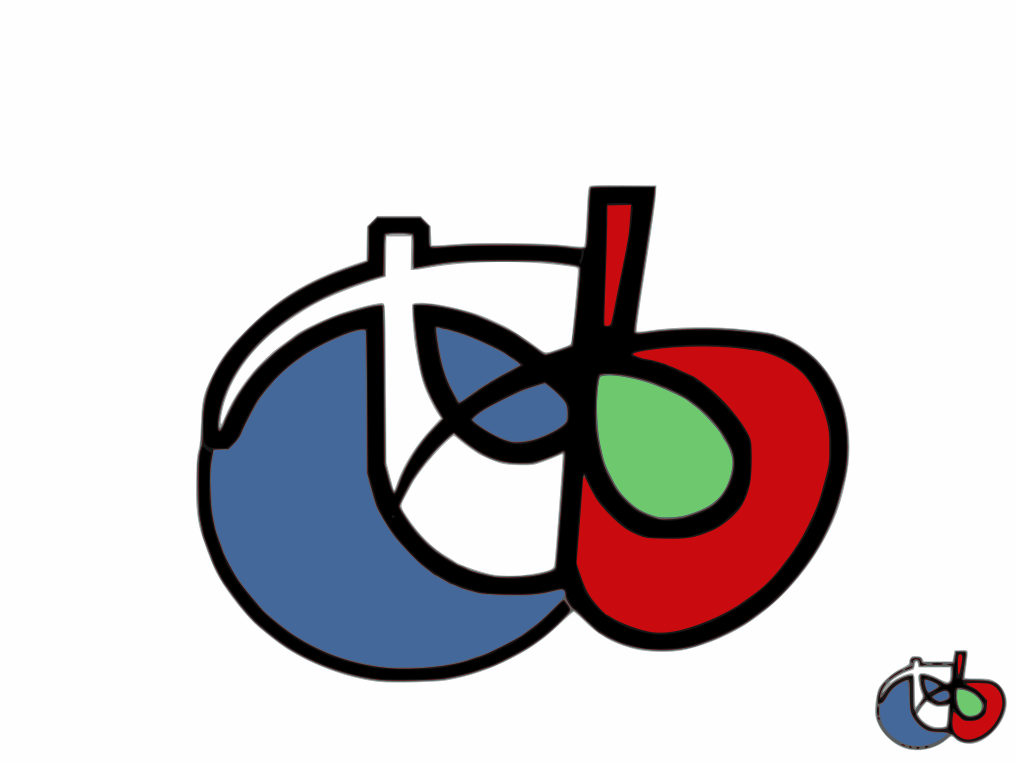
\includegraphics[width=0.7\columnwidth]{Pictures/logoVectoriel.png}\\	
	\end{flushleft}
\end{minipage}
\hfill
\begin{minipage}[c]{0.69\textwidth}
\begin{center}
\resizebox{0.7\linewidth}{!}{\textbf{\sc Orfeo ToolBox}}\\
\vspace{0.5cm}
\huge{\textcolor{red}{www.orfeo-toolbox.org}}\\
\vspace{0.7cm}
\Huge{\textbf{\sc open source remote sensing}}
\vspace{0.7cm}
%\url{orfeo-toolbox.org} 
\end{center}
\end{minipage}
\hfill 
\begin{minipage}[r]{0.15\textwidth}
	\begin{center}
		\vspace{1cm}
		\includegraphics[width=1.0\columnwidth]{Pictures/logo_cnes.jpg}\\		
	\end{center}
\end{minipage}

\vspace{1cm}


%%%%%%%%%%%%%%%%%%%%%
%%% BODY
%%%%%%%%%%%%%%%%%%%%%

\begin{minipage}[t]{\textwidth}
\titresection{\sc What is Orfeo ToolBox ?}
\vspace{0.5cm}
\begin{minipage}[t]{0.3\textwidth}
\titresubsection{Orfeo ToolBox in a nutshell}
\Large{
\begin{itemize}
\item It is an image processing library dedicated to remote sensing
\item It is a free and open source software under CeCILL v2 license (French equivalent
  to GPL)
\item It is funded and developed by CNES in the frame of the ORFEO acompaniement program
\item It is written in \verb!C++! on top of ITK (medical image processing)
\item It interfaces seamlessly with other image processing and remote
  sensing open-source softwares, like GDAL, OSSIM or OpenCV
\item Available on multiple platforms (Windows, Linux, Mac OS X)
\item It is scalable thanks to parallel and on the flow processing
\end{itemize}

\textcolor{red}{Thanks to its modular architecture, Orfeo ToolBox allows fast prototyping and development of processing-chains.}
\vspace{0.5cm}}
\end{minipage}
\hfill
\begin{minipage}[t]{0.3\textwidth}
\titresubsection{What you can do with Orfeo ToolBox}
\Large{
\begin{itemize}
\item Read, write, convert, extract parts of your remote sensing data,
\item Perform basic pre-processing like ortho-rectification, radiometric calibration or pan-sharpening,
\item Perform common image processing tasks (thresholding, Fourier or wavelets
  transform\ldots)
\item Extract features (radiometric indices, textures, shapes \ldots),
\item Segment images and vectorize segmentation results (at image scale),
\item Classify images in a supervised or unsupervised way,
\item Perform object-based image analysis,
\item Export results in Google Earth, QGIS and pretty print for publishing.
\end{itemize}
}
\end{minipage}
\hfill
\begin{minipage}[t]{0.3\textwidth}
\begin{minipage}[t]{\textwidth}
\titresubsection{Pleiades image in Orfeo ToolBox}
\Large{
\begin{itemize}
\item Supports JPEG 2000 image format through the open-source library OpenJPEG
\item Supports projection information and analytical sensor models through OSSIM
\item Supports calibration information to convert DN reflectance values to absolute radiance values
\item Decoding of intermediate resolutions
\item Efficient viewing and navigation with Monteverdi2 (see below)\\
\end{itemize}
}
\end{minipage}
\begin{minipage}[t]{\textwidth}
\titresubsection{\textcolor{red}{Getting help and support}}
\Large{
\begin{itemize}
\item As an open source software, OTB has its own users and developers
  community
\item The development team provides support through mailing-list
  (otb-users@googlegroups.com)
\item Features request can also be sent this way
\item Want to keep in touch with the OTB? Bookmark our blog (\url{blog.orfeo-toolbox.org})
\end{itemize}
}
\end{minipage}
\end{minipage}
\end{minipage}

\begin{minipage}[t]{\textwidth}
\titresection{\sc How can I use Orfeo ToolBox ?}
\vspace{0.5cm}
\begin{minipage}[t]{0.3\textwidth}
\titresubsection{By programming} \Large{Know a little about
  programming and want to access the full range of Orfeo ToolBox
  functions to build custom tools? Dive into our Software Guide and
  start writing your own \verb!C++! code with OTB. 

}

\end{minipage}
\hfill
\begin{minipage}[t]{0.3\textwidth}
\titresubsection{By running OTB applications} 

\Large{ Try our application
  plugins, shipped with a command-line interface, a Qt graphical
  interface and a Python (and other high-level languages) one for
  remote sensing tasks scripting.
}
\end{minipage}
\hfill
\begin{minipage}[t]{0.3\textwidth}
\titresubsection{By using Monteverdi2} 

\Large{ Want an integrated software for everyday life image
  manipulation or support for your training courses? Try Monteverdi2,
  our end-user software featuring a nice image viewer and a range of
  image processing modules based on OTB.
}

\end{minipage}
\end{minipage}

\vspace{1cm}

\begin{minipage}[t]{\textwidth}
\titresection{\sc What does Orfeo ToolBox look like ?}
\vspace{0.5cm}
\begin{minipage}[t]{0.33\textwidth}
%\vspace{-18cm}
\begin{minipage}[t]{\textwidth}
\titresubsection{A simple example of C++ OTB code}
\begin{lstlisting}[language=c++,breaklines=true,breakatwhitespace=true,frame = tb,framerule = 0.25pt,fontadjust,backgroundcolor={\color{listlightgray}},basicstyle = {\ttfamily\scriptsize},keywordstyle = {\ttfamily\color{listkeyword}\textbf},identifierstyle = {\ttfamily},commentstyle = {\ttfamily\color{listcomment}\textit},stringstyle = {\ttfamily},showstringspaces = false,showtabs = false,numbers = none,numbersep = 6pt, numberstyle={\ttfamily\color{listnumbers}},tabsize = 2]
#include "otbImage.h"
#include "otbImageFileReader.h"
#include "otbImageFileWriter.h"
#include "itkCannyEdgeDetectionImageFilter.h"
#include "itkRescaleIntensityImageFilter.h"

int main(int argc, char * argv[])
{
  typedef double                      PixelType;
  typedef otb::Image<PixelType>       ImageType;
  
  typedef unsigned char               OutputPixelType;
  typedef otb::Image<OutputPixelType> OutputImageType;

  typedef otb::ImageFileReader<ImageType> ReaderType;
  ReaderType::Pointer reader = ReaderType::New();

  reader->SetFileName(argv[1]);

  typedef itk::CannyEdgeDetectionImageFilter
  <ImageType, ImageType> FilterType;
  FilterType::Pointer filter = FilterType::New();

  filter->SetInput(reader->GetOutput());

  typedef itk::RescaleIntensityImageFilter
  <ImageType, OutputImageType> RescalerType;
  RescalerType::Pointer rescaler = RescalerType::New();

  rescaler->SetOutputMinimum(0);
  rescaler->SetOutputMaximum(255);

  rescaler->SetInput(filter->GetOutput());

  typedef otb::ImageFileWriter<OutputImageType> WriterType;
  WriterType::Pointer writer = WriterType::New();

  writer->SetFileName(argv[2]);
  
  writer->SetInput(rescaler->GetOutput());

  writer->Update();

  return EXIT_SUCCESS;
}
\end{lstlisting}
\end{minipage}
\vspace{1cm}
\begin{minipage}[t]{\textwidth}
\titresubsection{\textcolor{red}{How can I help ?}}
\Large{
We do not only need developers! To get involved, you can :
\begin{itemize}
\item Help us to validate algorithms and send feedback \url{bugs.orfeo-toolbox.org}
\item Provide OTB case studies (user stories)
\item Provide new ideas and feature requests
\item Help us improve the documentation
\item Spread the word !
\end{itemize}
}
\end{minipage}
\end{minipage}
\hfill
\begin{minipage}[t]{0.33\textwidth}
%\vspace{-18cm}
\begin{minipage}[t]{\textwidth}
\titresubsection{Calling applications from command-line}
\begin{lstlisting}[language=ksh,breaklines=true,breakatwhitespace=true,frame = tb,framerule = 0.25pt,fontadjust,backgroundcolor={\color{listlightgray}},basicstyle = {\ttfamily\small},keywordstyle = {\ttfamily\color{listkeyword}\textbf},identifierstyle = {\ttfamily},commentstyle = {\ttfamily\color{listcomment}\textit},stringstyle = {\ttfamily},showstringspaces = false,showtabs = false,numbers = none,numbersep = 6pt, numberstyle={\ttfamily\color{listnumbers}},tabsize = 2]
$ otbcli_ImageClassifier -in QB_1_ortho.tif -imstat clImageStatisticsQB1.xml -model clsvmModelQB1.svm -out classification.png uchar
\end{lstlisting}
\end{minipage}

\vspace{1.5cm}

\begin{minipage}[t]{\textwidth}
\titresubsection{Calling applications from Qt interface}
\begin{center}
\includegraphics[width=0.8\textwidth]{Pictures/qt_app.png}
\end{center}
\end{minipage}

\vspace{1.5cm}

\begin{minipage}[t]{\textwidth}
\titresubsection{Calling applications from Python}
\begin{lstlisting}[language=python,breaklines=true,breakatwhitespace=true,frame = tb,framerule = 0.25pt,fontadjust,backgroundcolor={\color{listlightgray}},basicstyle = {\ttfamily\footnotesize},keywordstyle = {\ttfamily\color{listkeyword}\textbf},identifierstyle = {\ttfamily},commentstyle = {\ttfamily\color{listcomment}\textit},stringstyle = {\ttfamily},showstringspaces = false,showtabs = false,numbers = none,numbersep = 6pt, numberstyle={\ttfamily\color{listnumbers}},tabsize = 2]
#!/usr/bin/python

# Import the otb applications package
import otbApplication

# The following line creates an instance of the ImageSVMClassifier application 
ImageSVMClassifier = otbApplication.Registry.CreateApplication("ImageClassifier")

# The following lines set all the application parameters:
ImageClassifier.SetParameterString("in", "QB_1_ortho.tif")
ImageClassifier.SetParameterString("imstat", "clImageStatisticsQB1.xml")
ImageClassifier.SetParameterString("model", "clsvmModelQB1.svm")
ImageClassifier.SetParameterString("out", "classification.png")
ImageSVMClassifier.SetParameterOutputImagePixelType("out", 1)

# The following line execute the application
ImageClassifier.ExecuteAndWriteOutput()
\end{lstlisting}
\end{minipage}
\end{minipage}
\hfill
\begin{minipage}[t]{0.33\textwidth}
\begin{minipage}[t]{\textwidth}
\titresubsection{Monteverdi2 viewer}
\begin{center}
\includegraphics[width=0.64\textwidth]{Pictures/monteverdi2-loupe.png}
\end{center}
\end{minipage}
\vspace{0.5cm}

\begin{minipage}[t]{\textwidth}
\titresubsection{Monteverdi2 Haralick Texture Extraction application}
\begin{center}
\includegraphics[width=0.64\textwidth]{Pictures/monteverdi2-haralick.png}
\end{center}
\end{minipage}
\vspace{0.5cm}

\begin{minipage}[t]{\textwidth}
\titresubsection{Monteverdi2 segmentation visualization}
\begin{center}
\includegraphics[width=0.64\textwidth]{Pictures/monteverdi2-segmentation.png}
\end{center}
\end{minipage}

\end{minipage}
\end{minipage}








\end{poster}
\end{document}
